\documentclass{standalone}
\usepackage{tikz}
\usepackage{verbatim}
\begin{document}
\pagestyle{empty}
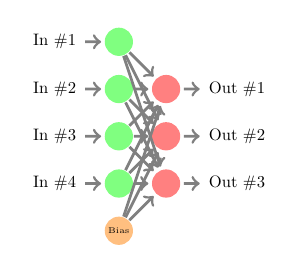
\begin{tikzpicture}[scale=0.6, transform shape, shorten >=1pt,->,draw=black!50, node distance=\layersep, line width=1pt]
    \tikzstyle{every pin edge}=[<-,shorten <=1pt]
    \tikzstyle{neuron}=[circle,fill=black!25,minimum size=17pt,inner sep=0pt]
    \tikzstyle{input neuron}=[neuron, fill=green!50];
    \tikzstyle{output neuron}=[neuron, fill=red!50];
    \tikzstyle{bias neuron}=[neuron, fill=orange!50];
    \tikzstyle{annot} = [text width=4em, text centered]
    % Draw the input layer nodes
    \foreach \name / \y in {1,...,4}
        \node[input neuron, pin=left:In \#\y] (I-\name) at (0,-\y) {};
    \node[bias neuron] (B-1) at (0,-5) {\tiny{Bias}};
    % Draw the output layer node
    \foreach \name / \y in {1,...,3}
        \path[yshift=-1cm]
            node[output neuron,pin={[pin edge={->}]right:Out \#\y}] (O-\name) at (\layersep,-\y cm) {};
    % Connect every node in the input layer with every node in the hidden layer.
    \foreach \source in {1,...,4}
        \foreach \dest in {1,...,3}
            \path (I-\source) edge (O-\dest);
    \foreach \dest in {1,...,3}
        \path (B-1) edge (O-\dest);
\end{tikzpicture}
\hfill
\column{0.4\textwidth}
\begin{tikzpicture}[
    thick, >=stealth', scale=0.45, transform shape,
    dot/.style = {draw,fill = white,circle,inner sep = 0pt,minimum size = 4pt}
  ]
  \coordinate (O) at (0,0);
  \draw[->] (-0.3,0) -- (6,0) coordinate[label = {below:$x$}] (xmax);
  \draw[->] (0,-0.3) -- (0,5) coordinate[label = {right:$t$}] (ymax);
  \path[name path=x] (0.3,0.5) -- (6.7,4.7);
  \path[name path=y] plot[smooth] coordinates {(-0.3,2) (2,1.5) (4,2.8) (6,5)};
  \draw[red] plot[smooth] coordinates {(-0.3,1) (2,1.6) (4,3.3) (6,4)};
  \draw (1,1.4) node[dot] {}  (3,2.7) node[dot] {} (5,3.4) node[dot] {};
  \draw[blue] (0,1) -- (6,4);
  \node[right] at (-2,2.5) {\Huge{$\simeq$}};
\end{tikzpicture}
\end{document}